\chapter{Implementazione}

\section{Breve descrizione del programma}
Per lo studio di quanto descritto fino ad ora si è costruito un programma in grado di caricare un file \lstinline{.wav} in buffer di dimensione arbitraria in memoria per poterne elaborare il contenuto; dopodiché è possibile specificare una catena di operazioni da effettuare sul segnale e un metodo di salvataggio del risultato (\lstinline{.wav} o \lstinline{.csv}). La catena di operazioni e il salvataggio vengono specificati in un file di testo. Per la lettura e scrittura su file .wav si utilizza la libreria ``libsndfile'' scritta da Erik de Castro Lopo \cite{libsndfile}.

L'invocazione del programma avviene tramite riga di comando ed è necessario utilizzare un programma esterno per visualizzare il contenuto dei file di output. I grafici dei risultati che verranno mostrati in questa tesi sono stati generati utilizzando un file \lstinline{.csv} in uscita dal programma il quale viene poi visualizzato tramite il programma Veusz \cite{veusz}.

\section{Strutture dati utilizzate}

Per la rappresentazione dei dati dei campioni in ingressi si utilizza una struttura nominata \lstinline{SignalBuffer_t} definita nel seguente modo:

\begin{lstlisting}
struct SignalBuffer_t
{
	cuComplex* samples;
	size_t channels;
	size_t* channel_size;
	size_t max_size;
};
\end{lstlisting}

Essa continene un array di campioni, il numero di canali, la lunghezza dei buffer di ogni canale e la lunghezza massima disponibile dell'array. I campioni sono organizzati nell'array di numeri complessi secondo lo schema descritto in figura \ref{fig:signalbuffersamples}, ovvero lo stesso modo in cui vengono restituiti i dati dalle funzioni di lettura di \lstinline{libsdnfile}.

\begin{figure}[h]
    \centering
    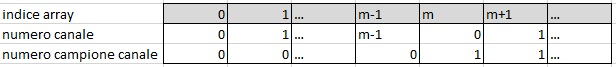
\includegraphics[width=1\textwidth]{signalbuffersamples}
    \caption{Disposizione dei campioni nella struttura \lstinline{SignalBuffer_t} supponendo $m$ canali.}
    \label{fig:signalbuffersamples}
\end{figure}

\lstinline{cuComplex} è un tipo importato dalla libreria di CUDA il quale rappresenta un numero complesso. Esso può essere utilizzato, con le apposite operazioni, sia dalla CPU sia dalla GPU.

Vengono definite anche operazioni su questa struttura, le quali garantiscono la corretta gestione dei campioni all'interno della stessa. Le funzioni utilizzate sono dichiarate con i modificatori \lstinline{__host__ __device__} i quali sono necessari al compilatore di CUDA per segnalare che tali funzioni possono essere sia eseguite sulla CPU (host), sia sulla scheda grafica (device).

\section{Convoluzione}
Il primo algoritmo che è stato studiato e implementato è la convoluzione tra segnali la quale è indispensabile perché è il primo strumento con cui si può calcolare la risposta di un sistema ad un determinato segnale se si conosce la risposta impulsiva del sistema stesso.

La definizione di convoluzione tra segnali discreti è descritta dall'equazione \ref{eq:convoluzionediscreta}. Bisogna porre particolare attenzione al fatto che la lunghezza del risultato della convoluzione è uguale alla somma delle lunghezze dei segnali in ingresso meno uno; questo comporta che bisogna far attenzione a gestire il fenomeno detto ``overlap'' tra buffer risultanti consecutivi; questo fenomeno, grazie alla linearità del sistema, si riduce solamente alla somma della ``coda'' del buffer in uscita precedente con i primi campioni del buffer in uscita seguente.

Visto che la convoluzione è una operazione che necessita di due segnali in entrata, si è supposto che il secondo segnale sia di un solo canale e non sia diviso in vari buffer, ma sia tutto contenuto in uno solo, mentre il primo segnale può essere diviso in più buffer. Questa decisione è giustificata dal fatto che spesso la convoluzione viene utilizzata tra un segnale molto lungo e uno di gran lunga più corto, poiché, come già detto, è una operazione onerosa in termini di calcolo. In particolare è spesso utilizzata per operazioni di filtraggio e in questo caso il secondo segnale prende il nome di ``kernel del filtro'' \cite[p.~108]{dspguide}. Nelle spiegazioni seguenti si utilizzerà la parola ``kernel'' per indicare il secondo segnale della convoluzione; bisogna prestare attenzione a non confondere il ``kernel'' del filtro con le funzioni ``kernel'' di CUDA.

\subsection{CPU}

La convoluzione sulla CPU è implementata utilizzando due cicli \lstinline{for}: uno che scorre i campioni del buffer in entrata di un determinato canale e l'altro invece che scorre i campioni del buffer contenente il secondo segnale. I due campioni ottenuti vengono quindi moltiplicati assieme e vengono poi aggiunti al valore di un buffer temporaneo. La presenza del buffer temporaneo è necessaria per la corretta gestione del fenomeno dell'``overlap''; il buffer temporaneo alla fine della convoluzione conterrà i campioni in uscita dalla convoluzione e la ``coda'' da sommare alla convoluzione successiva.

Una versione semplificata alle componenti fondamentali del codice che è stato utilizzato è il seguente:
\begin{lstlisting}
...
for (size_t i = 0; i < input_size; i++)
{
    cuComplex in_sample = get_sample(input, channel, i);
    for (size_t j = 0; j < kernel_size; j++)
    {
        size_t index = i+j;
        cuComplex kernel_sample = get_sample(kernel, SIGNAL_CHANNEL, j);
        cuComplex out_sample = get_sample(temp, channel, index);
        cuComplex result = cuCaddf(out_sample, cuCmulf(in_sample, kernel_sample));
        set_sample(temp, channel, index, result);
    }
}
...
\end{lstlisting}
Come si può osservare sono presenti i due cicli \lstinline{for} e le operazioni per effettuare l'accumulazione nel buffer temporaneo. Le funzioni \lstinline{cuCaddf} e \lstinline{cuCmulf} sono specificate da CUDA per effettuare rispettivamente la somma e il prodotto tra numeri complessi. È importante sapere che l'implementazione di \lstinline{get_sample} è scritta in modo che restituisca un numero complesso con parte reale e immaginaria uguali a $0$ (zero) nel caso l'indice richiesto sia fuori dalla dimensione dell'array del canale.

Questo tipo di implementazione viene chiamata da Smith ``algoritmo dal lato dell'ingresso'' \cite[pp.~112-115]{dspguide}, poiché elabora il contributo di ogni singolo elemento dell'ingresso rispetto a più posizioni nell'uscita.

In figura \ref{fig:pulse32conv} si può osservare il risultato della convoluzione di un impulso di 32 campioni con sé stesso ottenuto con l' algoritmo presentato.
\begin{figure}[h]
    \centering
    \subfloat[Impulso]{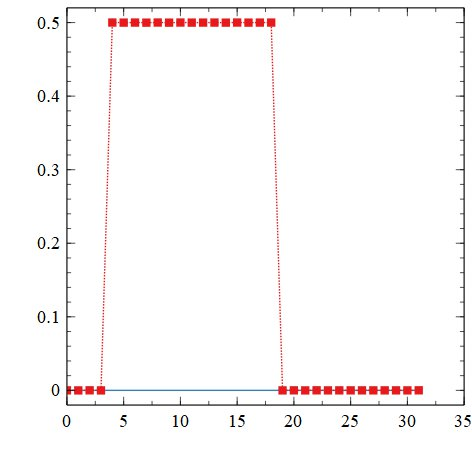
\includegraphics[width=0.5\textwidth]{pulse32}}
    \subfloat[Convoluzione]{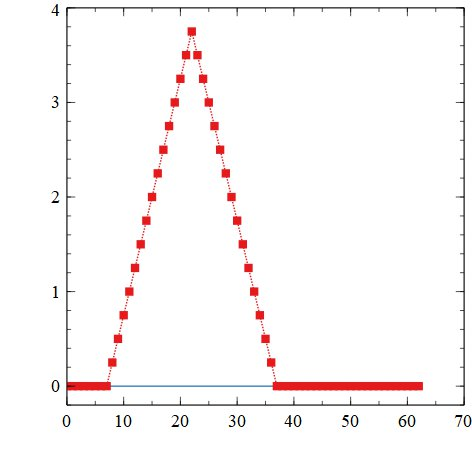
\includegraphics[width=0.5\textwidth]{pulse32conv}}
    \caption{Convoluzione di un impulso rettangolare con sé stesso. In rosso è segnata la parte reale e in blu la parte immaginaria}
    \label{fig:pulse32conv}
\end{figure}

\subsection{GPU}
Per implementare la convoluzione sulla GPU è necessario individuare i thread che è possibile parallelizzare e racchiuderli in uno o più kernel. Nel caso in esame si è deciso di utilizzare l'implementazione che Smith chiama ``algoritmo dal lato dell'uscita'' \cite[pp.~116-121]{dspguide}, il quale differisce dall'algoritmo precedentemente illustrato nell'implementazione sulla CPU per il fatto che si calcolano i contributi di vari campioni dell'ingresso rispetto ad un solo campione in uscita. I due algoritmi, seppur presentino due punti di vista diversi, sono equivalenti e restituiscono lo stesso risultato.

Bisogna prestare attenzione al fatto che dato un kernel di un filtro di $M$ elementi, il valore dell'elemento $i$-esimo dell'uscita è uguale al prodotto dell'elemento $i-j$ esimo dell'ingresso con l'elemento $j$-esimo del kernel del filtro, con $j = 0 ... M-1$.

Il kernel CUDA utilizzato per compiere questa operazione ridotto alle sue operazioni essenziali è il seguente:

\begin{lstlisting}
__global__ void cudaconvolver_kernel(SignalBuffer_t device_buffer, SignalBuffer_t kernel_buffer, SignalBuffer_t out_buffer, size_t channel)
{
    int k = blockIdx.x * blockDim.x + threadIdx.x;
    ...
    cuComplex temp_sample = make_cuComplex(0,0);
    for (int i = 0; i < kernel_size; i++)
    {
        kernel_sample =
            get_sample(kernel_buffer, SIGNAL_CHANNEL, i);
        input_sample =
            get_sample(device_buffer, channel, k-i);
        temp_sample = cuCaddf(temp_sample,
            cuCmulf(kernel_sample, input_sample));
    }
    set_sample(out_buffer, channel, index, temp_sample);
    ...
}
\end{lstlisting}

Si noti la presenza dell'indice $k$, il quale viene calcolato in base agli indici del thread corrente e del blocco corrente; esso identifica la posizione $k$ dell'elemento dell'uscita da calcolare. 

Se il segnale in ingresso è composto di $N$ punti e il kernel del filtro è composto da $M$ punti, il segnale in uscita è di $N+M-1$ punti; infatti la funzione kernel viene eseguita $N+M-1$, ovvero è presente una esecuzione della funzione per ogni elemento in uscita.

Nel codice mostrato è stato tolta la parte per la gestione dell'effetto di ``overlap'' in modo da rendere evidenti le parti fondamentali della sua implementazione per la GPU.

Il grafico in figura \ref{fig:convtime} rappresenta il tempo necessario per compiere una convoluzione utilizzando un kernel di un filtro di dimensioni fisse (128 punti) e facendo variare la lunghezza del file in ingresso da elaborare. Inoltre per quanto riguarda la GPU sono visualizzati anche valori diversi di lunghezza del buffer di elaborazione, in quanto, a differenza della CPU che non risente della grandezza dello stesso, la GPU presenta prestazioni via via migliori all'aumentare della dimensione del buffer, poiché un buffer più grande significa elaborare più dati in parallelo.
\begin{figure}[h]
    \centering
    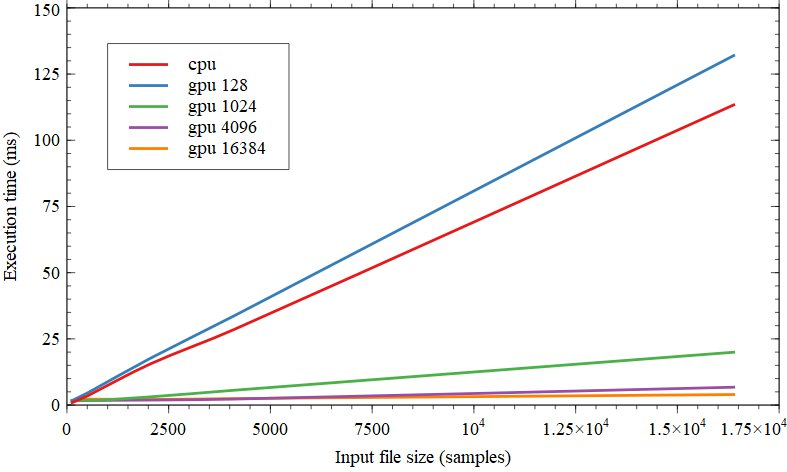
\includegraphics[width=\textwidth]{conv-time}
    \caption{Tempo di convoluzione, CPU e GPU a confronto}
    \label{fig:convtime}
\end{figure}

\section{DFT}
Un secondo algoritmo interessante da implementare è la trasformata di Fourier discreta. Essa trova larga applicazione come strumento di analisi spettrale dei segnali, oltre ad essere un punto di partenza per poi introdurre la \textit{Fast Fourier Transform} (FFT).

Come indicato nell'equazione \ref{eq:dft}, la DFT è sostanzialmente una sommatoria di un prodotto di numeri complessi, notiamo però che a differenza della equazione della convoluzione (\ref{ed:convoluzionediscreta}) il valore massimo della sommatoria dipende dalla lunghezza del segnale. Questo significa che nella implementazione saranno necessari due cicli \lstinline{for} innestati che dipendono entrambi dalla lunghezza del segnale. Tale configurazione di cicli \lstinline{for} restituisce una complessità computazionale di tipo $O(N^2)$. Motivo ulteriore per cui si è sviluppato l'algoritmo della FFT.

\subsection{CPU}
L'implementazione della trasformata di Fourier discreta è ricavata direttamente dalla sua equazione.

\begin{lstlisting}
void dft_wsio(SignalBuffer_t* bufferIn, SignalBuffer_t* bufferOut, size_t channel, size_t size)
{
    ...
    for (size_t k = 0; k < size; k++)
    {
        ...
        for (size_t i = 0; i < size; i++)
        {
            cuComplex s =
                cuComplex_exp(-2 * M_PI * k * i / size);
            cuComplex sample =
                get_sample(*bufferIn, channel, i);
            cuComplex outs =
                get_sample(*bufferOut, channel, k);
            outs = cuCaddf(outs, cuCmulf(sample, s));
            set_sample(*bufferOut, channel, k, outs);
        }
    }
    ...
}
\end{lstlisting}

\lstinline{cuComplex_exp(float x)} è una funzione che restituisce il numero complesso $e^{jx}$. L'algoritmo prende in input un buffer di cui effettuare la trasformata, un buffer in cui inserire il risultato della trasformazione, il canale dei buffer su cui operare e la dimensione in punti della trasformata. Come esposto in precedenza la funzione \lstinline{get_sample} restituisce il numero complesso $0$ nel caso il valore dell'indice sia fuori range. Questo permette di implementare facilmente la dft di un buffer con un pad di zeri alla sua destra.

\begin{figure}[h]
    \centering
    \subfloat[Impulso]{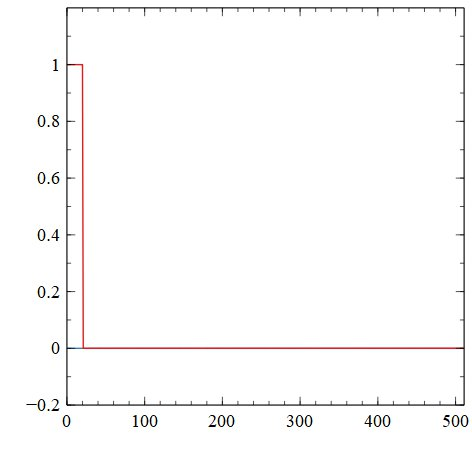
\includegraphics[width=0.5\textwidth]{pulse512}}
    \subfloat[Dft]{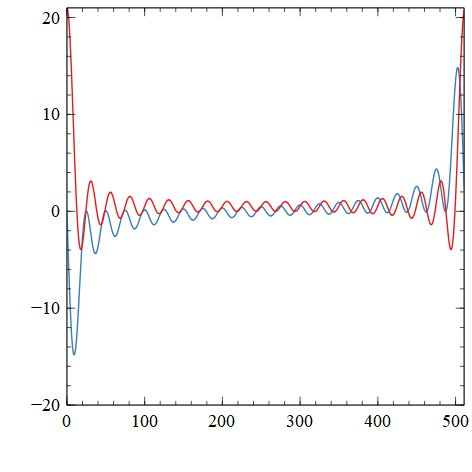
\includegraphics[width=0.5\textwidth]{pulse512dft}}
    \caption{DFT di un impulso di 512 campioni. In rosso è segnata la parte reale e in blu la parte immaginaria}
    \label{fig:pulse512}
\end{figure}

Inserendo nel programma l'impulso di 512 campioni mostrato in figura \ref{fig:pulse512}a si ottiene la trasformata in figura \ref{fig:pulse512}b. Come è facile notare, il segnale di partenza ha solo componente reale, quindi la sua trasformata è simmetrica rispetto a $N/2$ in modo pari per la parte reale e in modo dispari per la parte immaginaria.

\subsection{GPU}
L'operazione di trasformata di Fourier discreta è implementata sulla GPU utilizzando il seguente kernel:

\begin{lstlisting}
__global__ void cudadft_kernel_dft(SignalBuffer_t device_buffer, SignalBuffer_t out_buffer, size_t channel, size_t size)
{
    int k = blockIdx.x * blockDim.x + threadIdx.x;
    ...
    cuComplex temp = make_cuComplex(0, 0);
    for (int i = 0; i < size; i++)
    {
        cuComplex sample =
            get_sample(device_buffer, channel, i);
        cuComplex s
            = cuComplex_exp(-2.0f * PI * k * i / size);
        temp = cuCaddf(temp, cuCmulf(sample, s));
    }
    set_sample(out_buffer, channel, k, temp);
}

\end{lstlisting}

Anche in questo caso, il kernel viene eseguito in parallelo su tutti i campioni del segnale risultando più prestante della rispettiva implementazione sulla CPU. In particolare si può già notare che la complessità di ogni singolo thread si è ridotta a $O(N)$.

[grafici prestazioni]

\section{Fast Fourier Transform}
L'operazione di DFT è onerosa in termini di calcolo in quanto ha complessita $O(N^2)$, per cui si utilizza spesso la Fast Fourier Transform al suo posto (FFT). Uno degli algoritmi più popolari per il calcolo della FFT è quello ideato da Cooley e Tukey nel 1965. Esso fa uso della decomposizione interlacciata e delle somme a ``farfalla''.

[da espandere con più info]

\subsection{CPU}
La FFT è implementata sulla CPU nel seguente modo:

\begin{lstlisting}
    [codice da ridimensionare]
\end{lstlisting}

[da fare].

\subsection{GPU}

[da fare]
